\documentclass[11pt,a4paper]{article}

% Packages 
\usepackage[utf8]{inputenc}
\usepackage[T1]{fontenc}
\usepackage{lmodern}
\usepackage{graphicx}
\usepackage{amsmath, amssymb}
\usepackage{booktabs}
\usepackage{hyperref}
\usepackage[margin=1in]{geometry}
\usepackage{caption}
\usepackage{subcaption}
\usepackage{float}
\usepackage{placeins}

\hypersetup{
    colorlinks=true,
    linkcolor=blue,
    citecolor=blue,
    urlcolor=blue
}

% Title
\title{\textbf{Patent Reranking with Dense and Cross Encoders}}
\author{Md Naim Hassan Saykat}
\date{}

\begin{document}
\maketitle

\begin{abstract}
This project explores reranking methods for patent retrieval by combining dense retrieval with transformer-based cross-encoders. The pipeline integrates traditional TF--IDF baselines, dense embeddings (BGE), and cross-encoder re-ranking, further enhanced through Reciprocal Rank Fusion (RRF). Experiments on a patent dataset demonstrate improvements in retrieval quality measured by Mean Average Precision (MAP), Recall@k, and Mean Rank.
\end{abstract}

\noindent \textbf{Keywords:} Information Retrieval, Dense Retrieval, Cross-Encoder, Reranking, Patents, Reciprocal Rank Fusion.

% Introduction 
\section{Introduction}
Patent search is a critical task in information retrieval due to the large volume of documents and the need for precise relevance judgments. 
Classical term-based methods such as TF--IDF offer efficiency but suffer from lexical mismatch. 
Neural embedding models such as Dense Passage Retrieval (DPR) \cite{karpukhin-etal-2020-dense} and transformer-based re-rankers like BERT \cite{nogueira2019passage} have emerged as powerful solutions for capturing semantic relevance. 
Recent advances in open-source toolkits such as Hugging Face Transformers \cite{wolf2020transformers} have made it easier to integrate dense retrievers and cross-encoders into end-to-end IR pipelines. 
This project explores how these approaches can be combined and adapted for the patent retrieval domain.

This work implements and evaluates a reranking pipeline for patents, using a combination of:
\begin{itemize}
    \item TF--IDF (baseline),
    \item Dense retrieval with BGE embeddings,
    \item Cross-encoder re-ranking with a fine-tuned BERT model,
    \item Reciprocal Rank Fusion (RRF) for combining results.
\end{itemize}

% Methodology 
\section{Methodology}
\subsection{Dataset}
The dataset consists of patent queries, relevance mappings, and document features:
\begin{itemize}
    \item \texttt{train\_queries.json} – training queries
    \item \texttt{test\_queries.json} – test queries used for evaluation
    \item \texttt{train\_gold\_mapping.json} – relevance judgments
    \item \texttt{documents\_features.json} – patent document features
\end{itemize}
Due to GitHub file-size limits, the dataset is hosted externally on Google Drive.\footnote{\url{https://drive.google.com/drive/folders/1Oy4Gp1KVO__O1JnX1V4JuZ0zy7jlK78J?usp=sharing}}

\subsection{Models}
\begin{itemize}
    \item \textbf{TF--IDF Baseline:} Sparse vector retrieval for initial ranking.
    \item \textbf{Dense Retriever (BGE):} Embedding-based retrieval producing dense representations of queries and documents, inspired by prior dense retrieval work \cite{karpukhin-etal-2020-dense}.
    \item \textbf{Cross-Encoder:} A BERT-based pairwise scoring model trained on query--document pairs, following the passage re-ranking paradigm \cite{nogueira2019passage}.
    \item \textbf{Ensemble (RRF):} Reciprocal Rank Fusion combining dense retriever and cross-encoder outputs.
\end{itemize}

\subsection{Evaluation Metrics}
We report:
\begin{itemize}
    \item Mean Average Precision (MAP),
    \item Recall@10,
    \item Mean Rank.
\end{itemize}

Implementation of models and training pipelines was carried out using the Hugging Face Transformers library \cite{wolf2020transformers}.

% Experiments 
\section{Experiments}
\subsection{Training Setup}
The cross-encoder was trained using the \texttt{cross\_encoder\_reranking\_train.py} script with 3 epochs and batch size 16. Dense embeddings were precomputed using the BGE model. Evaluation scripts computed MAP, Recall@10, and Mean Rank.

\subsection{Results}
Table~\ref{tab:results} shows the retrieval performance across models. 
We also visualize the trends in Recall@10, MAP, and Mean Rank in Figure~\ref{fig:perf-comparison} 
for clearer comparison.

\begin{table}[H]
\centering
\begin{tabular}{lccc}
\toprule
\textbf{Model} & \textbf{MAP} & \textbf{Recall@10} & \textbf{Mean Rank} \\
\midrule
Dense Retriever (infly/inf-retriever-v1-1.5b) & 0.2140 & 0.4046 & 7.20 \\
Cross-Encoder Re-ranker & 0.2424 & 0.4426 & 6.35 \\
Ensemble (Dense + Cross-Encoder, RRF) & \textbf{0.2681} & \textbf{0.5321} & \textbf{4.90} \\
\bottomrule
\end{tabular}
\caption{Comparison of retrieval models on the patent dataset.}
\label{tab:results}
\end{table}

\FloatBarrier

\begin{figure}[H]
    \centering
    \begin{subfigure}{0.32\linewidth}
        \centering
        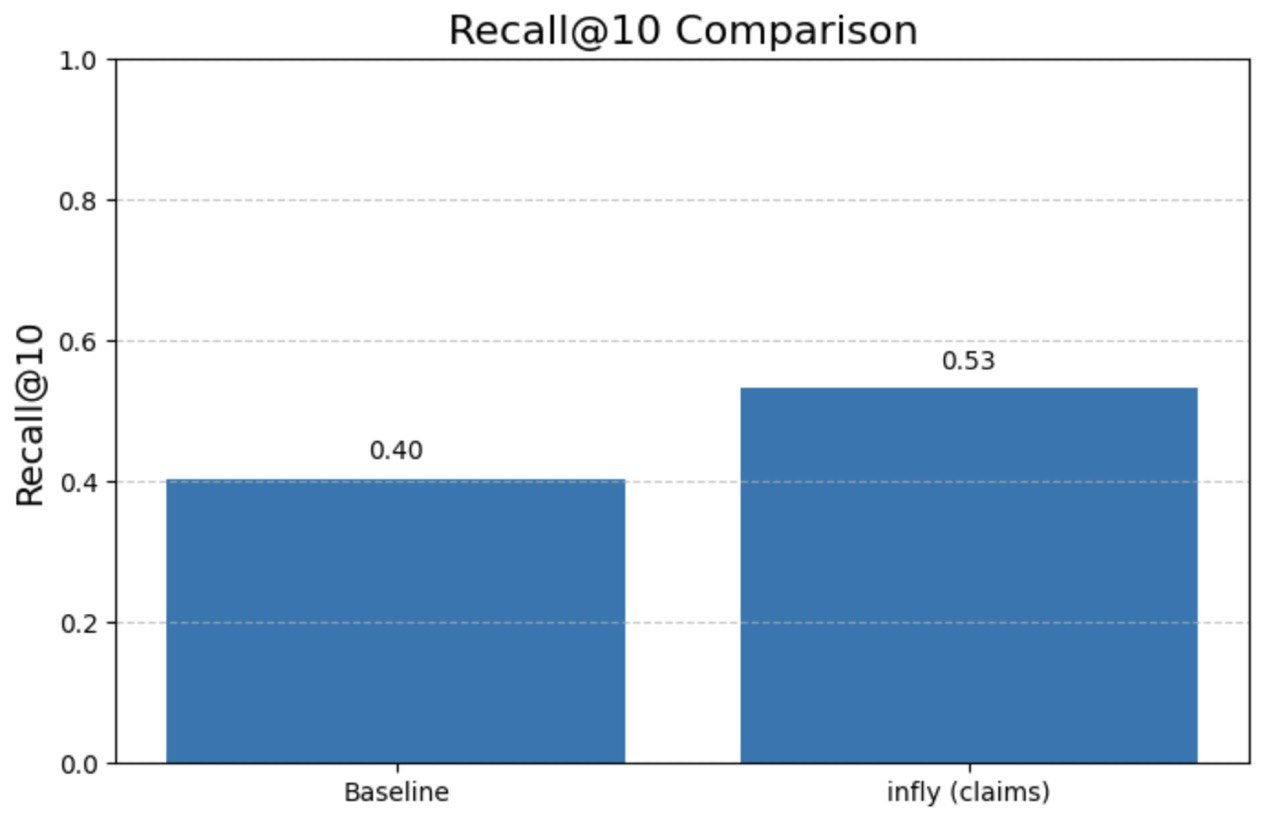
\includegraphics[width=\linewidth]{figs-recall10_comparison.png}
        \caption{Recall@10 Comparison}
    \end{subfigure}
    \hfill
    \begin{subfigure}{0.32\linewidth}
        \centering
        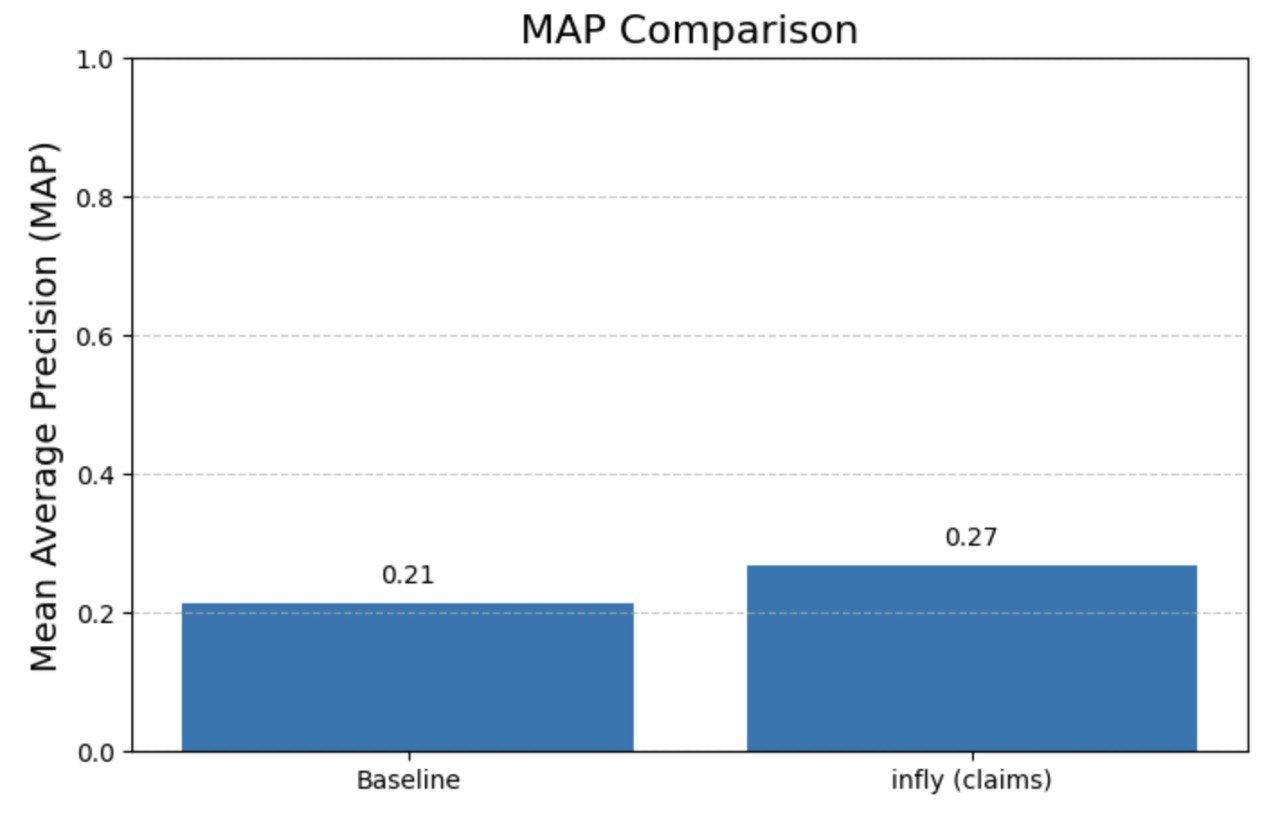
\includegraphics[width=\linewidth]{figs-map_comparison.png}
        \caption{MAP Comparison}
    \end{subfigure}
    \hfill
    \begin{subfigure}{0.32\linewidth}
        \centering
        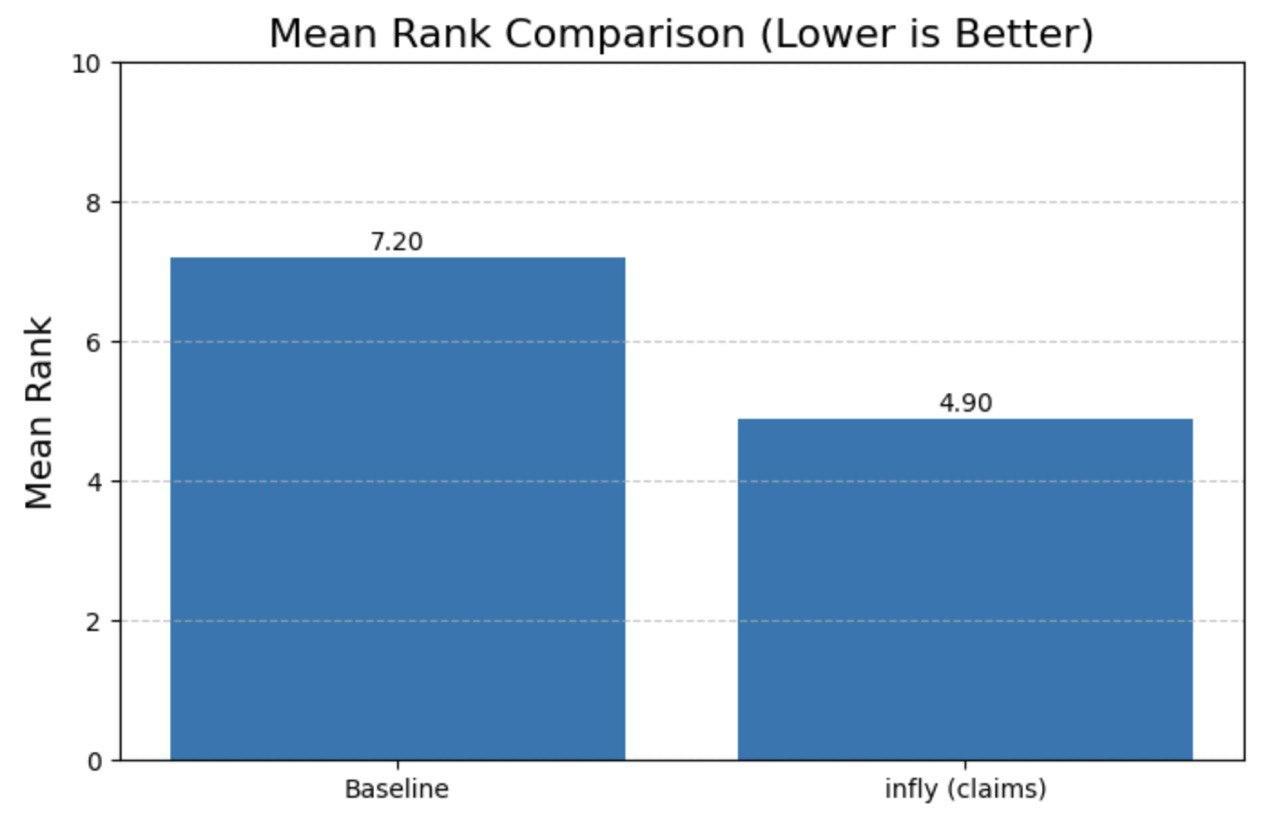
\includegraphics[width=\linewidth]{figs-meanrank_comparison.png}
        \caption{Mean Rank Comparison}
    \end{subfigure}
    \caption{Performance comparison across metrics: (a) Recall@10, (b) MAP, and (c) Mean Rank.}
    \label{fig:perf-comparison}
\end{figure}

% Discussion 
\section{Discussion}
The results in Table~\ref{tab:results} and Figure~\ref{fig:perf-comparison} highlight clear performance gains when moving from sparse to neural methods. 
The dense retriever improves over the baseline with a MAP of 0.2140 and Recall@10 of 0.4046, demonstrating the effectiveness of dense embeddings for semantic matching. 
The cross-encoder re-ranker further boosts performance, achieving MAP 0.2424 and Recall@10 0.4426, by explicitly modeling query--document interactions. 
Finally, the ensemble approach with Reciprocal Rank Fusion (RRF) yields the strongest results across all metrics (MAP 0.2681, Recall@10 0.5321, Mean Rank 4.90), confirming that hybrid methods effectively leverage complementary strengths. 
These findings indicate that while dense retrieval provides strong semantic coverage, combining it with re-ranking strategies maximizes both recall and ranking quality.
 
% Conclusion 
\section{Conclusion}
We developed and evaluated a patent reranking pipeline combining TF--IDF, dense retrievers, and cross-encoders, with further improvements from Reciprocal Rank Fusion (RRF). 
The results show that dense retrievers provide strong semantic matching, while cross-encoders further improve ranking by modeling fine-grained query--document interactions. 
The ensemble approach achieved the best overall performance (MAP 0.2681, Recall@10 0.5321, Mean Rank 4.90), confirming the effectiveness of hybrid pipelines that integrate retrieval and re-ranking strategies. 

This study highlights the value of combining complementary IR techniques to address patent search, where both semantic coverage and precise ranking are crucial. 
Future work could explore larger transformer-based re-rankers (e.g., DeBERTa, Longformer), domain-specific pretraining, and metrics such as nDCG and precision@k to further validate performance.

% References 
\bibliographystyle{plain}
\bibliography{references}

\end{document}